% TODOs: skontrolovat indexovanie, polo-otvorene intervaly, pridat viac prikladov pre succinct DS 

\chapter{Introduction to succinct data structures}
\label{kap:kap1}

\section{Motivation}

In many applications, the amount of data is so significant that our choice of
the data structures we use is heavily influenced by their space usage. The field
of \textit{succinct data structures} focuses on representing data using as little
space as possible but at the same time tries not to hurt the time complexity and
performance of methods that these structures support. In this field, many data structures
for varied problems have been devised such as succinct dictionaries~\citep{raman2007succinct},
succinct trees (Fenwick tree by \cite{bille2017succinct}, trie by \cite{grossi2015fast}),
graphs \citep{farzan2013succinct} or text collections \citep{ferragina2000opportunistic}.
While many of the resulting structures come with solid theoretical bounds on the used space,
others look into real-world space usage and performance.

Succinct data structures are very helpful in scenarios where we work with a massive amount of
data. In these scenarios, using the ordinary data structures may force us to place
the entire representation of data structure onto the slower type of memory storage, thus
reducing the usability of our data structure and often completely ruining its runtime due to
high amount of slow \textit{I/O operations}. Even if a succinct version of the data structure
may help us to store the data in a faster type of memory (e.g. fast RAM instead of the slower disk),
we pay some price for using the succinct data structure. It comes mostly in the form of more
complex implementation.

In this work, we are mainly concerned with \textit{bit vector}. One of the simplest
data structures that represents a sequence of zeroes and ones while supporting the
following methods:
\begin{itemize}
\item $\access(i)$ - returns the $i$-th symbol of the sequence,
\item $\rank_c(i)$ - returns the number of occurrences of symbol $c$up to the $i$-th index
\item $\select_c(i)$ - returns the index of $i$-th occurrence of symbol $c$ in the sequence.
\end{itemize}

The reason behind our focus on bit vector and particularly its compressed version
is that it is one of the main building blocks of many succinct data structures.
In the next sections, we introduce some of its interesting and useful applications.

\section{Application 1: Sparse array}

Let $A$ be an array of $N$ elements each taking $k$ bits of space. We shall be interested in
accessing the $i$-th element of $A$. For simplicity, we assume that the elements of the array may
not change after the construction. A straightforward representation of this array takes $N\cdot k$
bits of space. However, imagine a scenario where a significant portion of the array is empty
and just a handful of elements are present. Take for example a sparse vector of numbers,
where most of the elements are 0. Then we could use a more space-efficient approach.
Let us assume that only $n$ out of $N$ elements are present and also that $n\ll N$.

First approach using the sparseness of an array is to store only the non-default elements as
pairs $(\text{position}, \text{value})$, which takes $n\cdot (k+\ceil{\log n})$ bits of space.
If we just store the pairs sorted by the position, accessing the $i$-th element takes $O(\log n)$ time.

We may use a hash table to obtain a constant time solution but this comes with additional
memory overhead.

An alternative approach using the bit vector is to store non-default elements in
a packed array $P$ of length $n$ and size $nk$ bits. Alongside $P$ we store a bit vector $B$ of length
$N$ where
\[
   B[i]=
\begin{cases}
   1,& \text{if $A[i]$ is occupied} \\
   0,& \text{if $A[i]$ is empty/default value.}
\end{cases}
\]

Using this representation of $A$, if we want to access the $i$-th element, we first check for
the value of $B[i]$. If it is zero, we return the default value. If it is one, we need to find
how many ones are preceding this particular one in $B$ to locate where our value is placed in
array $P$. For this, we may use the $\rank_1$ method. Similarly, to obtain the position of $i$-th
non-empty value in $A$, we use $\select_1$.


The total space used by this representation is $N+n\cdot k+R$ where $R$ is the space needed to
support an efficient $\rank$ query. As we shall show in Section~\ref{section:rank}, $\rank$ can
be implemented in constant time with sublinear space overhead, i.e., $R = o(N)$. If we are provided
with bit vector implementation along with $\access$ and $\rank$ methods we are able to reduce the
total space used from $k\cdot N$ to $N+n\cdot k+o(N)$ bits. Note that in practice, for a really small
number of non-default values, the hashtable representation takes up less space, however, bit
vector provides us with a solution that is usable for scenarios when $A$ is mediumly filled in,
e.g. $n/N>0.10$.

\section{Application 2: Storing elements of non-uniform length}

Let us consider another problem of representing an array of elements that are of variable length.
This type of elements can often arise in succinct data structures when trying to
optimise the amount of space used. An example of this is a \textit{Huffman code} \citep{huffman1952method}
that constructs the optimal code for symbols based on the symbol frequencies. More frequent
symbols are assigned shorter code while less frequent symbols get longer code.
Even though we can store these elements one after another in memory, with the variable-length
elements, we do not have an easy and fast way to tell where is the $i$-th element located.

Let us assume that we have $n$ elements of variable length. The first solution is to allocate
the array of length $nk_{MAX}$ bits where $k_{MAX}$ is the number of bits used for the element
with the longest bit representation. This enables constant time access but wastes a lot of space.

A second possible solution is to allocate a bit array $R$ where the elements are stored one after
another in their raw bit representation. To locate the $i$-th element we store alongside $R$ a
helper array $P$. Number on $i$-th position is the index where the $i$-th element begins in $R$.
This helper array consumes at least $\Theta(n\log n)$ bits as every entry contains an index into
the array $R$.

The helper array $P$ can be replaced by a bit vector of the same length as is $R$, storing ones at
positions where some element in $R$ begins (see an example in Fig.~\ref{obr:VariableSizedElements}).
Identifying the beginning of the $i$-th element now boils down to efficiently locating the
$i$-th one in the helper bit vector, which can be answered using the $\select_1$ method.
In Chapter~\ref{kap:kap2}, we shall see how this method can be implemented efficiently.

\begin{figure}
	\centerline{
	\begin{tabular}{l|l|l|l|l|l|l|l|l|l|l|}
	\cline{2-11}
	\textbf{Raw binary representation} & 1          & 1 & 0 & 1 & 1          & 1 & 1          & 0 & 1 & 0          \\ \cline{2-11} 
	\textbf{Beginnings of an elements}          & \textbf{1} & 0 & 0 & 0 & \textbf{1} & 0 & \textbf{1} & 0 & 0 & \textbf{1} \\ \cline{2-11} 
	\end{tabular}
	}
	\caption[TODO]{Raw binary representation of elements 1101, 11, 101 and 0 stored one after another.
	Note the helper bit array that is of the same size with ones on the positions where new element begins.}
	\label{obr:VariableSizedElements}
\end{figure}

\section{Application 3: FM-index}
% sources to help understand https://www.dcc.uchile.cl/TR/2005/TR_DCC-2005-004.pdf

Let us now consider practically more interesting application within a more complex data structure.
As we shall see, solution
to this problem also uses bit vector and other building blocks commonly used in succinct
data structures. This time, we have a text $T$ and we are interested in \textit{indexing} it.
After preprocessing text, we would like to quickly answer questions such as “how many times is
some pattern $P$ contained in $T$“ and also “where in $T$ are these occurrences located“.

This is particularly useful in bioinformatics, where we have a very long sequence of DNA and
are interested in searching for some subsequences in it such as a \emph{read mapping}
\citep{simpson2010efficient} problem.

One of the solutions that is reasonably fast and may be used is constructing a \textit{suffix array}
of $T$. Suffix array of $T$ is a data structure that stores information about the lexicographical
order of suffixes of $T$. More precisely, on $i$-th position of suffix array $S$, it stores the
starting position of suffix that comes $i$-th in lexicographical order. An example of suffix array is in
Fig.~\ref{obr:suffixArray}. For simplicity, in this section, we assume that every text
$T$ contains a special character {\tt \$} located only at its end that is lexicographically
smaller than any other character contained in $T$. Searching for pattern $P$ in suffix array of $T$ uses fact that
if $P$ is contained in $T$ it will be at the beginning of some suffixes that make up a
continuous subsequence of $S$.

\textit{FM-index}, proposed by \cite{ferragina2000opportunistic} is a succinct data structure that
is in some aspects similar to suffix array. FM-index can find the pattern in the preprocessed text
in time complexity close to linear from $|P|$. Its space usage depends on the compressibility of the text but the
resulting space used by FM-index is in many cases smaller than the space used for the original text $T$.
For instance, FM-index over the DNA sequence can take just 30--40\% of the space taken by the original text
$T$ as was observed by \cite{ferragina2001experimental}.

In the rest of this section, let us now explain how the FM-index is constructed, how we search in an
FM-index and how/why FM-index uses rank computation on general strings, which are implemented via
wavelet trees based on bit vectors.

\paragraph{Burrows-Wheeler transformation}

\textit{Burrows-Wheeler transformation~(BWT)} proposed by \cite{burrows1994block} is a pivotal
part of the FM-index. BWT of a text $T$ gives us a sequence $\mathit{T_{BWT}}$ of the same
length. Furthermore, this operation is reversible in a sense that we are able to reconstruct
the original text $T$ only using $\mathit{T_{BWT}}$. This transformation is used as a
preprocessing step of some compression algorithms such as \textit{bzip2} introduced by
\cite{seward1996bzip2} and was studied more by \cite{manzini2001analysis}. This is because
BWT is oftentimes easier to compress. We shall show how it is constructed and then give 
intuition why it has this property.

Consider a sequence $T$ of symbols over some
alphabet $\Sigma$. Take all the cyclical rotations $T_1, T_2, \ldots ,T_n$ of
$T$ and imagine putting them sorted by their lexicographical order into the
rows of table $M$ as seen in Fig.~\ref{obr:BWT}. We name the sequence created by the
concatenation of symbols in first and last column $F$ and $L$, respectively. Last column $L$
is what we call the BWT of $T$. Note that the sequence $F$ can be obtained from $L$ just by
sorting all the characters in $\mathit{T_{BWT}}$. $F$ consists of runs of symbols that are
sorted according to the lexicographical ordering of alphabet symbols. We shall use the helper
sequence $\Count$ where $\Count[c]$ is number of occurrences of symbols smaller than $c$.
Note that the run of symbol $c$ in $F$ starts at the index $\Count[c]$.

\begin{figure}
	\centerline{
	\begin{tabular}{l|c|ccccc|c|}
	\cline{2-8}
	  & $F$ & \multicolumn{5}{l|}{} & $L$   \\ \cline{2-8} 
	0 & {\tt \$}	& \multicolumn{1}{c|}{{\color[HTML]{C0C0C0} \tt b}}		& \multicolumn{1}{c|}{{\color[HTML]{C0C0C0} \tt a}}	& \multicolumn{1}{c|}{{\color[HTML]{C0C0C0} \tt n}}	& \multicolumn{1}{c|}{{\color[HTML]{C0C0C0} \tt a}}	& {\color[HTML]{C0C0C0} \tt n}  & {\tt a}  \\ \cline{2-8} 
	1 & {\tt a}  		& \multicolumn{1}{c|}{{\color[HTML]{C0C0C0} \tt \$}} 	& \multicolumn{1}{c|}{{\color[HTML]{C0C0C0} \tt b}}	& \multicolumn{1}{c|}{{\color[HTML]{C0C0C0} \tt a}}	& \multicolumn{1}{c|}{{\color[HTML]{C0C0C0} \tt n}}	& {\color[HTML]{C0C0C0} \tt a}  & {\tt n}  \\ \cline{2-8} 
	2 & {\tt a}		& \multicolumn{1}{c|}{{\color[HTML]{C0C0C0} \tt n}}		& \multicolumn{1}{c|}{{\color[HTML]{C0C0C0} \tt a}}	& \multicolumn{1}{c|}{{\color[HTML]{C0C0C0} \tt \$}}& \multicolumn{1}{c|}{{\color[HTML]{C0C0C0} \tt b}}	& {\color[HTML]{C0C0C0} \tt a}	& {\tt n}  \\ \cline{2-8} 
	3 & {\tt a}		& \multicolumn{1}{c|}{{\color[HTML]{C0C0C0} \tt n}}		& \multicolumn{1}{c|}{{\color[HTML]{C0C0C0} \tt a}}	& \multicolumn{1}{c|}{{\color[HTML]{C0C0C0} \tt n}}	& \multicolumn{1}{c|}{{\color[HTML]{C0C0C0} \tt a}}	& {\color[HTML]{C0C0C0} \tt \$}	& {\tt b}  \\ \cline{2-8} 
	4 & {\tt b}		& \multicolumn{1}{c|}{{\color[HTML]{C0C0C0} \tt a}}		& \multicolumn{1}{c|}{{\color[HTML]{C0C0C0} \tt n}}	& \multicolumn{1}{c|}{{\color[HTML]{C0C0C0} \tt a}}	& \multicolumn{1}{c|}{{\color[HTML]{C0C0C0} \tt n}}	& {\color[HTML]{C0C0C0} \tt a}  & {\tt \$} \\ \cline{2-8} 
	5 & {\tt n}		& \multicolumn{1}{c|}{{\color[HTML]{C0C0C0} \tt a}}		& \multicolumn{1}{c|}{{\color[HTML]{C0C0C0} \tt \$}}& \multicolumn{1}{c|}{{\color[HTML]{C0C0C0} \tt b}}	& \multicolumn{1}{c|}{{\color[HTML]{C0C0C0} \tt a}}	& {\color[HTML]{C0C0C0} \tt n}  & {\tt a}  \\ \cline{2-8} 
	6 & {\tt n}		& \multicolumn{1}{c|}{{\color[HTML]{C0C0C0} \tt a}}		& \multicolumn{1}{c|}{{\color[HTML]{C0C0C0} \tt n}}	& \multicolumn{1}{c|}{{\color[HTML]{C0C0C0} \tt a}}	& \multicolumn{1}{c|}{{\color[HTML]{C0C0C0} \tt \$}}& {\color[HTML]{C0C0C0} \tt b}  & {\tt a}  \\ \cline{2-8} 
	\end{tabular}
	\hspace{4em}
	\begin{tabular}{l l l}
		sorted suffixes\\
	\hline
		\tt \$ \\
		\tt a\$ \\
		\tt ana\$ \\
		\tt anana\$ \\
		\tt banana\$ \\
		\tt na\$ \\
		\tt nana\$ \\
	\end{tabular}
	}
	\caption[TODO]{On the left we can see the matrix $M$ filled with cyclic rotations of sequence
	$S = \mathtt{banana\$}$. On the right, we can see the sorted suffixes (content of suffix array). The
	Burrows-Wheeler transformation of $S$ is string $L=\mathtt{annb\$aa}$ -- the last column of $M$.
	Note that in practice, we do not need to construct the whole table as more efficient algorithms exist.
	It is also notable that matrix $M$ includes very similar information to suffix array.
	}
	\label{obr:BWT}
\end{figure}

BWT is usually more compressible than the original text because it frequently contains runs of the same
symbol. This can be better explained on an example. Consider us having BWT of a text containing
a lot of mentions of the word {\tt home}. All the rotations prefixed with {\tt ome} will form a
continuous subsequence of rows of $M$. Some of these rows will end in {\tt c} for word {\tt come},
some of them in {\tt m} for {\tt moment} but many of these lines will contain {\tt h} at the end as this
is very common symbol preceding {\tt ome} in the text.

\paragraph{Searching in an FM-index}

As we already stated, FM-index is used for searching in the preprocessed text.
Searching in FM-index is based on the two important properties:

\begin{enumerate}
	\item Rotations starting with $w$ form a consecutive subsequence of rows in $M$.
	\label{chapter1:fmindexprop:prop1}
	\item The $i$-th occurence of character $c$ in $F$ corresponds to the $i$-th occurence of $c$ in~$L$.
	\label{chapter1:fmindexprop:prop2}
\end{enumerate}

The first property was also what enabled us to search for a pattern in a suffix array. The second
property is less trivial to observe. Let us take two rows in $M$, namely $T_i$ and $T_j$
such that $i<j$. Let $T_i$ be of the form $cA$ and $T_j$ of the form $cB$ where $c$ is a
character from the text and $A$ and $B$ are sequences of characters. Since $i<j$, it follows that
$A<B$ and this means that rotated rows $Ac$ and $Bc$ are in the same order as original rows.
From this observation, we get that the relative ordering of the same character is maintained
from $F$ to $L$.

The search for rows where pattern $P$ is located proceeds from the end of $P$. This works by
finding rows where suffixes $P[n-1\ldots], P[n-2\ldots]$ etc. are located. In every step, these
rows will form a continuous subsequence of rows of $M$ so we store only its beginning and end.
This follows from the observation \ref{chapter1:fmindexprop:prop1}. Let us assume that we are
looking for a word {\tt house} and we already found the range of rows in $M$ that have {\tt ouse}
as their prefix. If we look to the last column in this range, these symbols correspond to the symbols
preceding {\tt ouse} in the text. We can maybe observe there in arbitrary order symbols like {\tt m}
for word {\tt mouse} or {\tt h} for {\tt house}. To search for the range of rows in $M$ that have as a prefix
word ({\tt house}) we look into the range of all prefixes beginning with {\tt h}. Locating this
range is easy thanks to the $\Count$ helper array. Lines in this range are sorted according to the
second character so there will be some lines continuing with {\tt a} if the text contained for example
word {\tt hashtag} or {\tt e} if the word {\tt head} was in the text. Somewhere the lines starting with 
{\tt house} will be located, but we do not store anything except for $T_{BWT}$ and $\Count$.
However, we already located the range where suffixes starting with {\tt ouse} are located in.
We can look how many times {\tt h} is located before this range in $T_{BWT}$. Thanks to this
number and the property \ref{chapter1:fmindexprop:prop2}, we know where in $F$ the subsequence
containing the prefix {\tt house} begins. 

% TODO: mozno obrazok
% TODO: fixnut indexovanie

In general, we first find the subsequence of $M$s rows, where suffix $P[n-1\ldots]$ is located.
As this is just a one symbol, $P[n-1]$, the initial subsequence is just a run of symbol $P[n-1]$
in $F$ given by
\begin{align*}
	b_{n-1}&=\Count[P[n-1]] \\
	e_{n-1}&=\Count[P[n-1]+1].\\
\end{align*}

The next step is to find where the subsequence of $M$s rows, given by $b_{n-2}$ and $e_{n-2}$ is located,
that has as a prefix $P[n-2\ldots]$. As we already located rows beginning with $P[n-1\ldots]$, we can reuse
this information. In a range from $b_{n-1}$ to $e_{n-1}$ some rows end with character $P[n-2]$. These are rows
that after being rotated, create subsequence we are looking for. Subsequence we are looking for is also
subsequence of a run of character $P[n-2]$ in $F$, starting from $\Count[P[n-2]]$ spanning rows up to
$\Count[P[n-2]+1]$. To find the offset of beginning and end of our subsequence along this run, we compute the
number of occurences of character $P[n-2]$ in $L$ up to the $b_{n-1}$, the start of previous subsequence of
rows and also the number of occurences of character $P[n-2]$ in $L$ up to the $e_{n-1}$ giving us its end.
This works thanks to the property \ref{chapter1:fmindexprop:prop2}. Thus giving us the new subsequence
\begin{align*}
	b_{n-2}&=\Count[P[n-2]] + \rank_{P[n-2]}(b_{n-1}) \\
	e_{n-2}&=\Count[P[n-2]] + \rank_{P[n-2]}(e_{n-1}).\\
\end{align*}
We continue and repeat the previous step until we compute $b_0$ and $e_0$ or until $b_i=e_i$ for some $i$
(in which case the searched word is not present in the text).

% TODO: pseudocode

The most important fact from this application is that we are not only interested in $\rank$ over a bit vector
and $\rank$/$\select$ functionality over general aphabet has particular use case in the FM-index. In the part
of this section, we show how we can reduce this problem with general alphabet to bit sequence version and
solve it using $\rank$ and $\select$ on bit vectors.

\paragraph{Wavelet tree}
\label{section:WaweletTree}

Assume for a moment that we have a bit vector implementation supporting methods $\access$,
$\rank$ and $\select$. Our goal is to build a vector over a general alphabet $\Sigma$
supporting the same three methods. The most straightforward approach to do this is to
have one bit vector $B_c$ for every character $c$ from alphabet $\Sigma$, storing ones at
positions where $c$ occurs in $S$
\[
    B_c[j]= 
\begin{cases}
	1,& \text{if } S[j]=c \\
    0,& \text{otherwise.}
\end{cases}
\]

This is indeed very fast because each $\rank$ and $\select$ operation can be answered using
only a single binary $\rank$ or $\select$. However, we use roughly $|\Sigma|$ times more space
than the single bit vector over this sequence.

\textit{Wavelet tree} uses a divide-and-conquer approach. It takes the sequence $S$ of
length $n$ over some alphabet $\Sigma$ and recursively splits the alphabet into
two subsets creating a hierarchical partitioning of an alphabet. In the root node
of the tree, it splits the alphabet $\Sigma$ into two subsets $\Sigma_0$ and $\Sigma_1$
of roughly equal size. It then stores a bit vector $B$ of size $n$ in this node
where
\[
    B[i]= 
\begin{cases}
    0,& \text{if } S[i]\in \Sigma_0\\
    1,              & \text{otherwise.}
\end{cases}
\]

Then it creates two strings $S_0$ and $S_1$ from $S$ by taking just symbols
from $\Sigma_0$ and $\Sigma_1$, respectively. The left and right children of the root node
are then built by recursively applying the same idea on subsequences $S_0$ and $S_1$ until
we end up with a trivial unary alphabet at the leaves. It follows that the depth of the
wavelet tree is $\ceil{\log |\Sigma|}$.
\begin{figure}
	\centerline{
		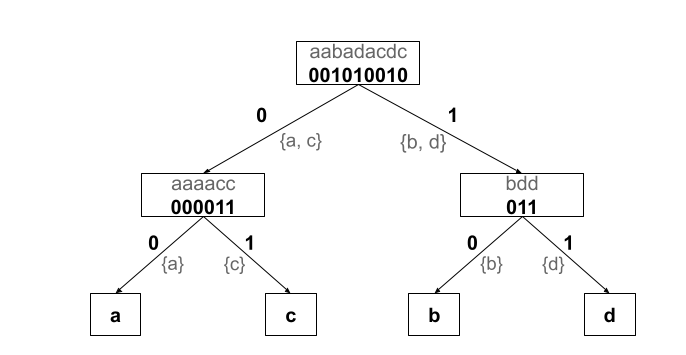
\includegraphics[width=0.9\textwidth, height=0.3\textheight]{images/wavelet_tree}
	}
	\caption[TODO]{Wavelet tree representation of text $S=\mathit{aabadacdc}$. We can see how
	the recursive partitioning of the alphabet works. In every node, we also show the
	subsequence represented (grey text) in the subtree of the node. The stored data can be
	recognized as they are in bold and black.
	}
	\label{obr:WaveletTreeExample}
	% based on https://simongog.github.io/assets/data/sdsl-slides/tutorial#23
	% source at https://docs.google.com/drawings/d/1cJyda3bdTluajr3iXu1x1iL5HF0JPZqAHw6jwct9KLI/edit
\end{figure}
Both $\rank_c$ and $\select_c$ methods on the original sequence can be implemented
using $\rank$/$\select$ methods applied on bit sequences that are along the path
from the root to the leaf containing character $c$. It follows that the number of
$\rank$ and $\select$ queries on individual bit vectors depends on the depth of
a leaf containing queried character $c$.

If we assign to every node except the root a {\tt 0} if it is the left son and {\tt 1}
otherwise, we can look at the wavelet tree as an assignment of a binary code to every
alphabets character. Code of a character $c$ in some leaf node is equal to concatenation of
bits that are contained in nodes on a path from root to the leaf node. The idea proposed
by~\cite{makinen2005succinct} is to shape the wavelet tree in such a way that a code of every
character is equal to Huffman code of this character.

% TODO: ze vyska je log n, aj v pripade Huffmana; average depth u Huffmana (ak by sme pristupovali k pismenam podla ich frekvencie, je H_0)
% TODO: chcelo by to nejaky sumar, lebo uz z toho mam nafuknutu hlavu: Cize: Hladanie v FM-indexe potrebuje rank a rank v stringu sa robi cez wavelet a ten pouziva rank na bitvektoroch (pripadne, ze v kapitole 4 ukazeme, ako zlepsenie bitvektorov zlepsi vyhladavanie v FM-indexe 
% TODO: chyba pojednanie o pamatovej zlozitosti: 1. wavelet stromzabera +/- tolko, co povodny text, 2. ak stlacime bitvektory na H_0, tak wavelet strom bude mat H_0(S) + cosi, 3. kolko zabera FM-index? za istych okolnosti H_k (+ citacie ku vsetkemu)

\section{Space efficiency}

There are many ways to measure the space efficiency of a data structure. From the
practical point of view, we may be interested in the memory usage by the data
structure on actual data that the structure could encounter in our use case. However,
many succinct data structures are trying to achieve some upper bounds and express
the used space in terms of the information contained in the data. There are many
models how to measure the information contained in sequences of characters. One
of the most commonly used models in the field of succinct data structures, yet still
quite simple, is entropy or more specifically zeroth-order entropy:

$$H(S)=\sum_{c\in\Sigma} \frac{n_c}{n} \lg \frac{n}{n_c}$$.

In many scenarios, where succinct data structures are used, the stored sequence
is compressible using the sole fact that some symbols have a bigger frequency than others.